%\chapter{Sensor and Weapon Models}
\section{Sensor and Weapon Models}
\label{sec:sensor_wpn_models}
UAVs carry sensors and weapons.  Sensors are used for scanning the world to determine if a target is present.  If a target is found sensors are then used for tracking the target.  Weapons are used for destroying targets.  There are multiple types of sensors and multiple types of weapons in the simulation.  Each has unique characteristics.  Each type of UAV carries a specific payload package of sensors and weapons.  This allows the UAVs to specialize as surveillance platforms, strike platforms, or multi-role platforms.
% \textbf{TODO: Should detect vs confirm be described here or in UAV models?}

%\section{Payload Type Definitions}
\subsection{Payload Type Definitions}

Each type of sensor in the simulation has a minimum and maximum detection range.  In reality any target that is too close would oversaturate a sensor and yield invalid results.  Any target that is too far away does not produce enough of a signal to be detectable.  This phenomena is modeled by bounding the valid detection range of the sensors.  Sensors can be mounted on a gimbal turret or in a fixed orientation on their host UAV.  If they are gimbaled the sensors cannot slew faster than a maximum slew rate that is unique to the sensor type. The performance characteristics of the sensors used in this simulation are shown in Table~\ref{tab:sensorType}.

\begin{table}[H]
	\caption{Sensor type definitions}
	\centering
	\rowcolors{1}{lightgray}{white}
	\label{tab:sensorType}
	\begin{tabular}{|p{1cm}|p{1.5cm}|p{1cm}|p{1cm}|p{1.5cm}|}
		\hline
		Sensor Type & Field of View ($^{\circ}$) & Min Range (m) & Max Range (m) & Slew rate ($\frac{^{\circ}}{s}$)\\ \hline
		0 & 60 & 10 & 1100 & 30 \\  \hline
		1 & 45 & 50 & 700  & 10 \\  \hline
	\end{tabular}
\end{table}

%Sensors have two scanning modes.  The normal mode is a wide angle scan set to a fixed field-of-view unique to the sensor type as shown in figure~\ref{fig:wide_angle_scan}.  The second mode is a focused scan of a small area.  This mode is meant to emulate a sensor that is zoomed in on something of interest.  This mode is used to confirm target identities and perform battle damage assessment in the simulation as shown in figure~\ref{fig:narrow_scan}.

The sensors in the simulation have two scanning modes.  The normal mode is a wide angle scan set to a fixed field-of-view unique to the sensor type.  The wide angle scan mode is used for general world observation.  The second mode is a focused scan of a small area.  This focused scan mode is meant to emulate a sensor that is zoomed in on something of interest.  This mode is used to confirm target identities and perform battle damage assessment in the simulation.  Figure~\ref{fig:scan_sizes} shows a UAV in the bottom right performing a wide area scan and another UAV in the center of the image performing a focused scan on a recently destroyed target.  Note the size difference between the sensor footprints rendered in yellow.


\begin{figure}[H]
	\centering
	%	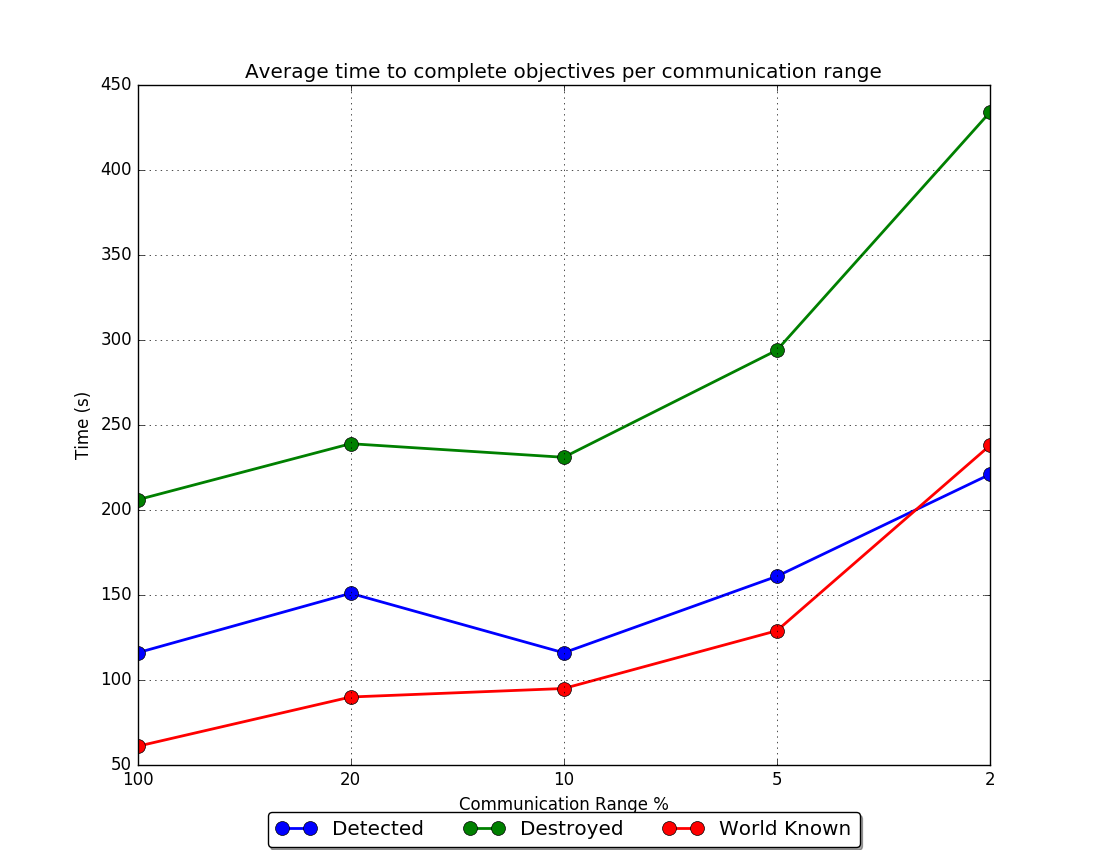
\includegraphics[width=\linewidth,height=4in,keepaspectratio=false]{averages.png}
	%	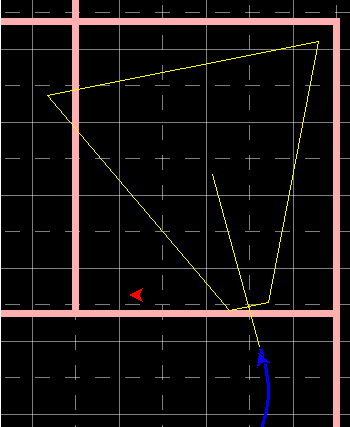
\includegraphics[scale=0.27]{wide_angle_scan.png}
	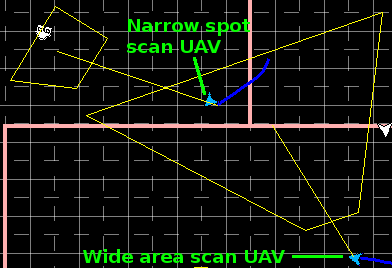
\includegraphics[width=\linewidth]{scan_sizes.png}
	\caption{Comparison of sensor footprints}
	\label{fig:scan_sizes}
\end{figure}

%\begin{figure}[H]
%	\centering
	%	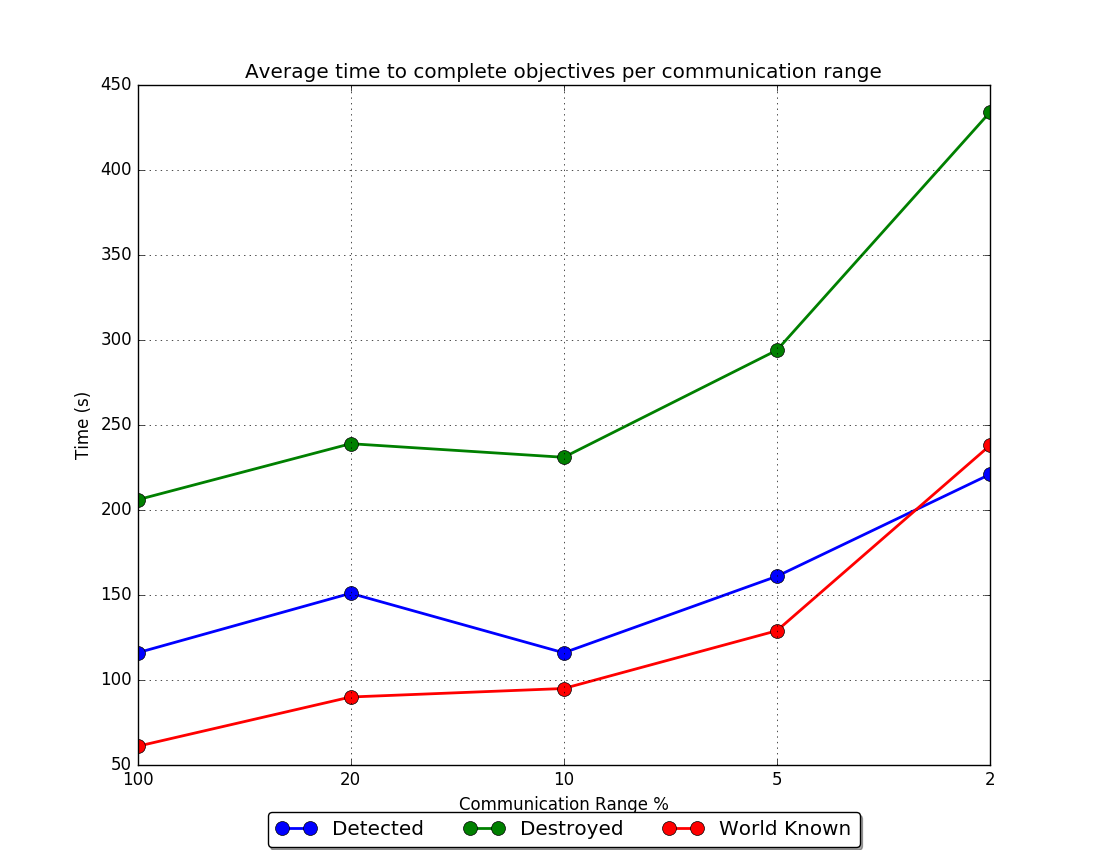
\includegraphics[width=\linewidth,height=4in,keepaspectratio=false]{averages.png}
%	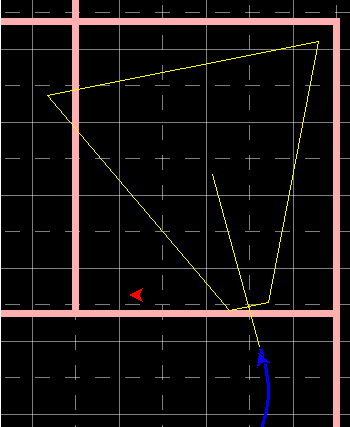
\includegraphics[scale=0.27]{wide_angle_scan.png}
%	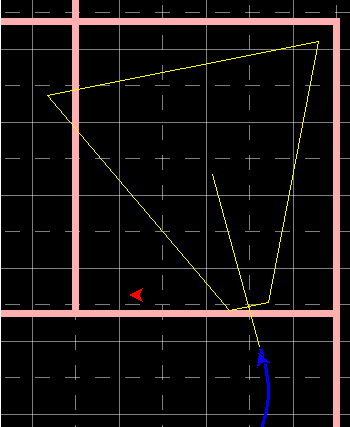
\includegraphics[width=\linewidth]{wide_angle_scan.png}
%	\caption{A sensor performing a normal wide angle area scan.}
%	\label{fig:wide_angle_scan}
%\end{figure}

%\begin{figure}[H]
%	\centering
	%	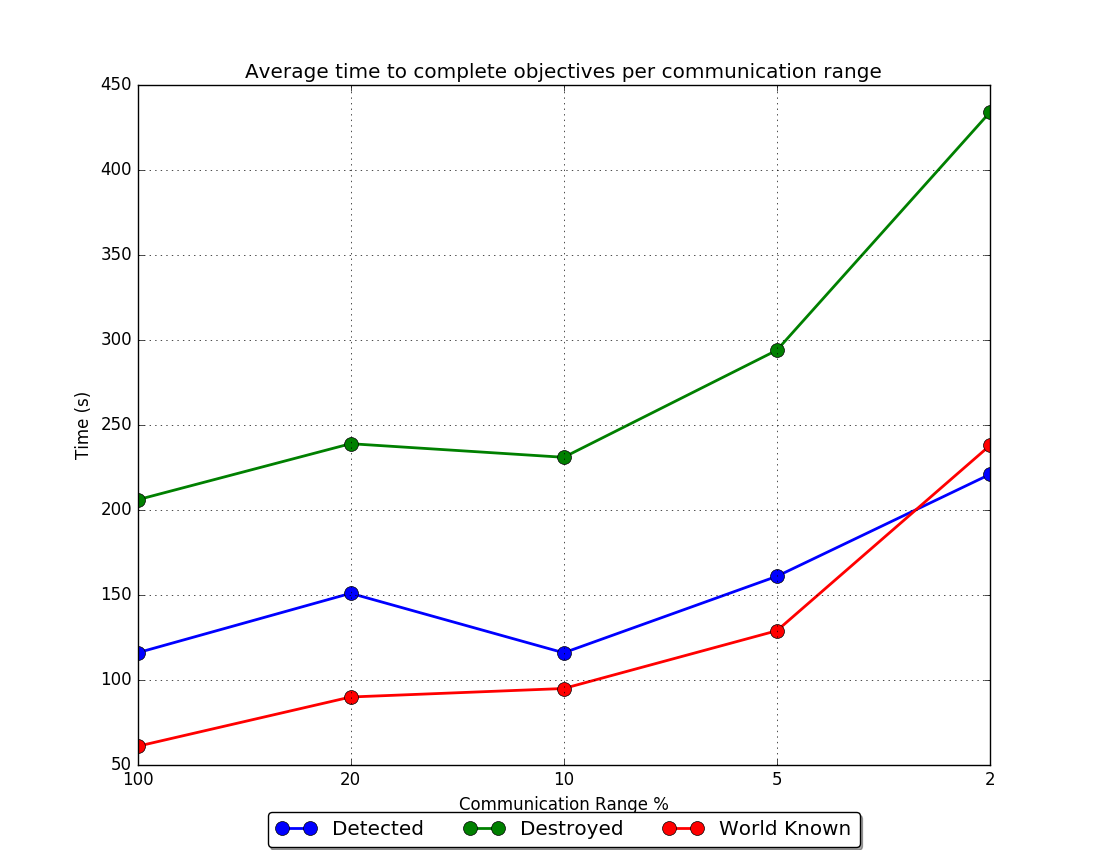
\includegraphics[width=\linewidth,height=4in,keepaspectratio=false]{averages.png}
	%	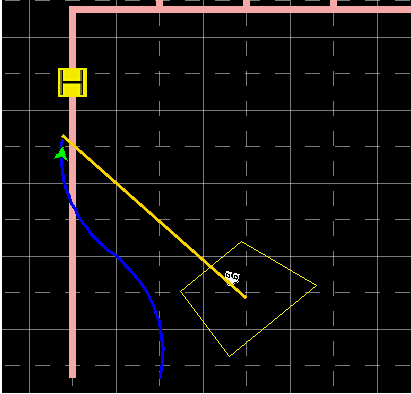
\includegraphics[scale=0.27]{narrow_scan.png}
%	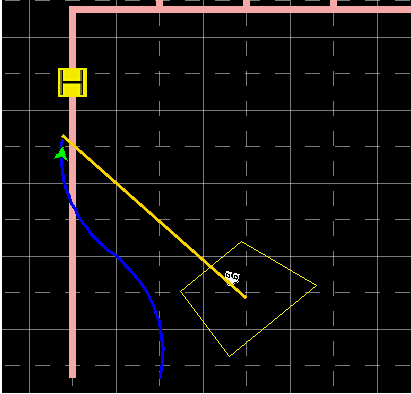
\includegraphics[width=\linewidth]{narrow_scan.png}
%	\caption{A sensor performing a focused narrow scan of a destroyed target}
%	\label{fig:narrow_scan}
%\end{figure}

Similarly, each weapon type has a minimum and maximum launch range.  If a target is too close the weapon will not have enough time to properly acquire the target and fuse itself.  If a target is too far away the weapon's propulsion system will fall short of a lethal distance.  Weapons have limited steering capabilities so the host UAV must align its heading to the target within an acceptable launch angle region. A sample set of data characterizing weapons can be seen in Table~\ref{tab:weaponType}.  The launch angle region is defined as the area between two bearings referenced to the left and right of the heading of the UAV.  For example in Table~\ref{tab:weaponType} weapon type 0 has a Launch Angle of $12^{\circ}$.  This means the bearing referenced from the nose of the UAV (boresight) to the target must be between $-12^{\circ}$ and $12^{\circ}$ before the UAV can launch the weapon.

% \todo{Do we care about a UAV being in the blast radius?}

\begin{table}[H]
	\caption{Weapon type definitions}
	\centering
	\rowcolors{1}{lightgray}{white}
	\label{tab:weaponType}
	\begin{tabular}{|p{1.4cm}|p{1.6cm}|p{1.2cm}|p{1.2cm}|}
		\hline
		Weapon Type & Launch Angle ($^{\circ}$) & Min Range (m) & Max Range (m)\\ \hline
		0 & 12 & 10 & 200 \\ \hline
		1 & 26 & 25 & 500 \\ \hline
	\end{tabular}
\end{table}

%\section{Payload Probabilities}
\subsection{Payload Probabilities}
\label{sec:payload_probs}

\subsubsection{Detecting Targets}
\label{sec:sensor_var_descriptions}
This simulation uses realistic sensors in that they cannot perfectly detect targets or clear areas.  Each type of sensor has a probability of detecting if a target exists, a probability for mistakenly detecting a target incorrectly, and an affinity for correctly estimating the heading of a target.  All of these attributes are user configurable and stored in lookup tables.  The values used for the experiment described in this paper are shown in Table~\ref{tab:snsrTgtProb} and Table~\ref{tab:snsrTgtMisClassProb}.  $P(S_{x}|T_{x})$ is the probability of a sensor $S$ detecting target type $x$ and correctly perceiving it as a type $x$.  $P(S_{j}|T_{i})$ is the probability of a sensor $S$ detecting target type $i$ and mistakenly perceiving it as a type $j$.  $H_{ij}$ is the Heading Estimation Coefficient for sensor $i$ against target type $j$.  It is purely a simulation construct used to help generate noise from truth data for sensor detections.  The $H_{ij}$ is not used in any UAV logic.  A value of zero for $H_{ij}$ means the sensor is near useless for estimating target headings while a value of one for $H_{ij}$ means the sensor can perfectly detect the target's heading.

$P(S_{x}|T_{x})$ and $P(S_{j}|T_{i})$ are defined assuming perfect alignment with the target's \textit{Best Angle}.  Any variance from the target's \textit{Best Angle} will cause these probabilities and heading estimates to degrade.  For example, if a visible light spectrum camera is viewing a person's front we can see their face.  From this angle we can detect that we are looking at a person and confirm their identity.  If we orbit around behind the person we can still detect that a person is in front of the camera but the probability of confirming their identity correctly falls.

\begin{table}[H]
	\caption{Sensor to Target Probabilities}
	\centering
	\rowcolors{1}{lightgray}{white}
	\label{tab:snsrTgtProb}
	\begin{tabular}{|p{1.2cm}|p{1.2cm}|p{1.5cm}|p{1cm}|}
		\hline
%		Sensor Type & Target Type & Prob(Detect) & Heading Estimation Coefficient\\ \hline
		Sensor Type & Target Type & $P(S_{x}|T_{x})$ & $H_{ij}$\\ \hline
		0 & 0 & 0.6 & 0.5 \\  \hline
		0 & 1 & 0.6 & 0.5 \\  \hline
		1 & 0 & 0.4 & 0.5 \\  \hline
		1 & 1 & 0.4 & 0.5 \\  \hline
	\end{tabular}
\end{table}

\begin{table}[H]
	\caption{Sensor to Target Misclassification Probabilities}
	\centering
	\rowcolors{1}{lightgray}{white}
	\label{tab:snsrTgtMisClassProb}
	\begin{tabular}{|p{1cm}|p{1.25cm}|p{1.6cm}|p{1.5cm}|}
		\hline
		Sensor Type & True Target Type & Perceived Target Type & $P(S_{j}|T_{i})$\\ \hline
		0 & 0 & 1 & 0.1 \\ \hline
		0 & 1 & 0 & 0.1 \\ \hline
		1 & 0 & 1 & 0.1 \\ \hline
		1 & 1 & 0 & 0.1 \\ \hline
	\end{tabular}
\end{table}

Figure~\ref{fig:targetAngles} shows the gradient of performance scaling around a target based on the offset from the \textit{Best Angle}.  In this figure the target has a \textit{Best Angle} of $45^{\circ}$ off of the target's front.  Any sensing or attacks at this angle, or its symmetric mirror at $315^{0}$, will function with $100\%$ normal performance as defined in the probability lookup tables.  The direct opposite location at $225^{\circ}$, or its mirror at $135^{0}$, has approximately a $50\%$ scaling value.  Any sensing or attack activities at these angles will have their performance cut in half.  Angles in between the \textit{Best Angle} and the opposite side will have their probabilities of success scaled by some percentage.

The scaling values in this model were derived assuming that a perfect alignment provides $100\%$ performance and an alignment exactly $180^{0}$ opposite provides $0\%$ performance.  Using a linear scale and the two end points just described yields a performance degradation slope of $-1 / 180$ as computed in Equation~\ref{eq:best_angle_degrade_slope}. However, due to the symmetric nature of the \textit{Best Angle} attribute the scaling performance never actually reaches $0\%$ since the best scaling from either mirror side is used.  At worst the scaling drops to $\approx30\%$ in Figure~\ref{fig:targetAngles}. 

\begin{equation}
\label{eq:best_angle_degrade_slope}
slope = \frac{0 - 1}{180-0} = \frac{-1}{180} \approx -0.0055556\frac{\%}{^{0}}
\end{equation}

%\end{multicols}

\begin{figure}[H]
	\centering
	%	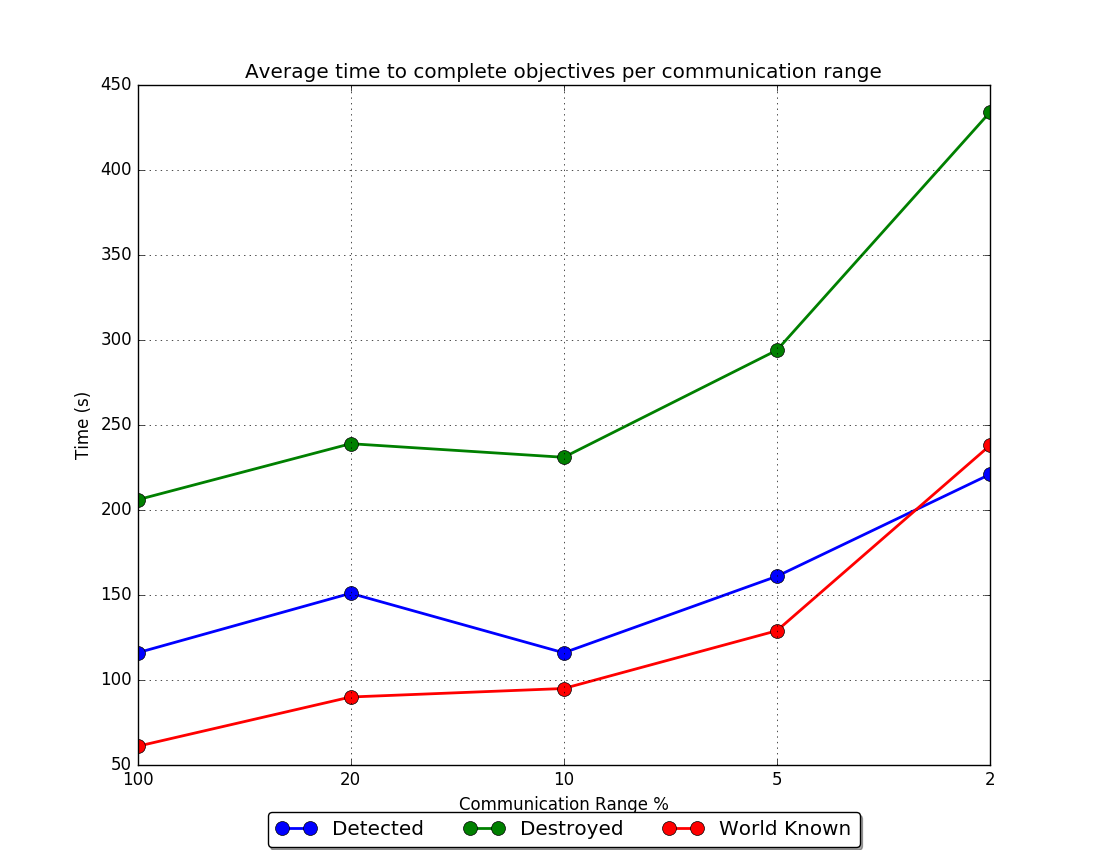
\includegraphics[width=\linewidth,height=4in,keepaspectratio=false]{averages.png}
	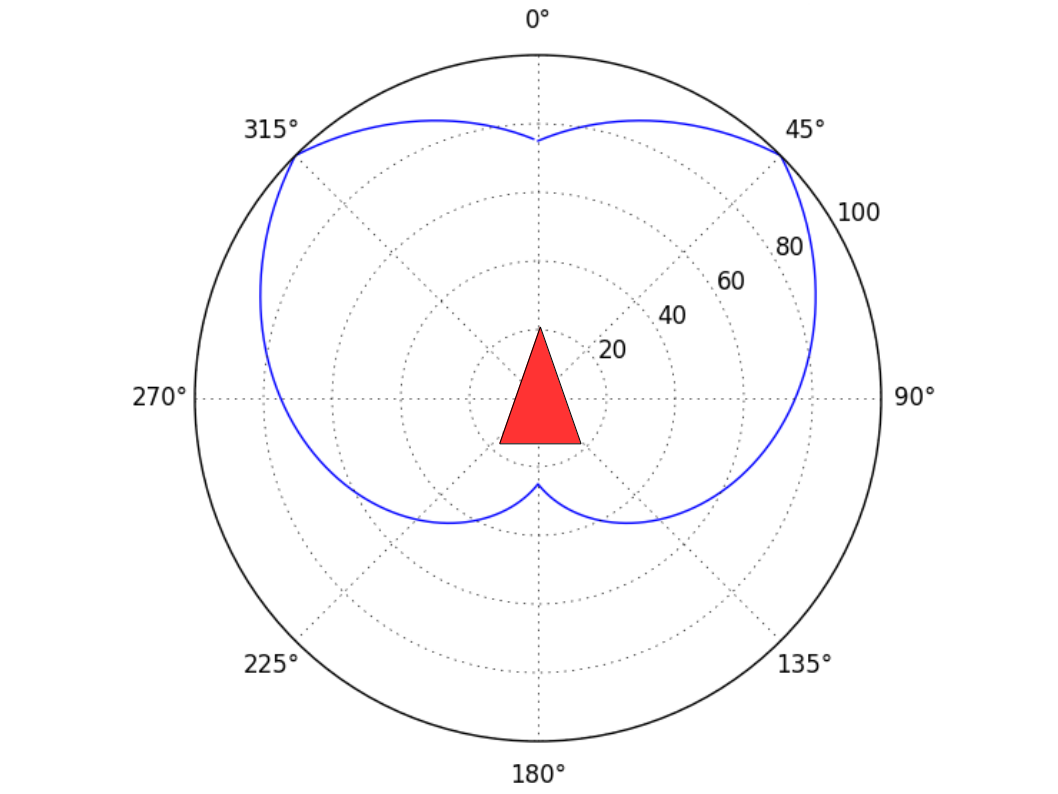
\includegraphics[scale=0.3]{red_scale_angle.png}
	\caption{Success scaling for a target with a \textit{Best Angle} of $45^{\circ}$}
	\label{fig:targetAngles}
\end{figure}

Figure~\ref{fig:blue_red_angles} shows an example of two UAVs in blue interacting with a red target.  The relative angle between the target's heading and Blue 1's is close to the \textit{Best Angle} of $45^{\circ}$.  Blue 1 can sense or attack the target with little to no performance degradation.  The relative angle between the heading of the target and Blue 2 is much greater.  Therefore, Blue 2 will suffer a degradation in sensing and attack performance.

\begin{figure}[H]
	\centering
	%	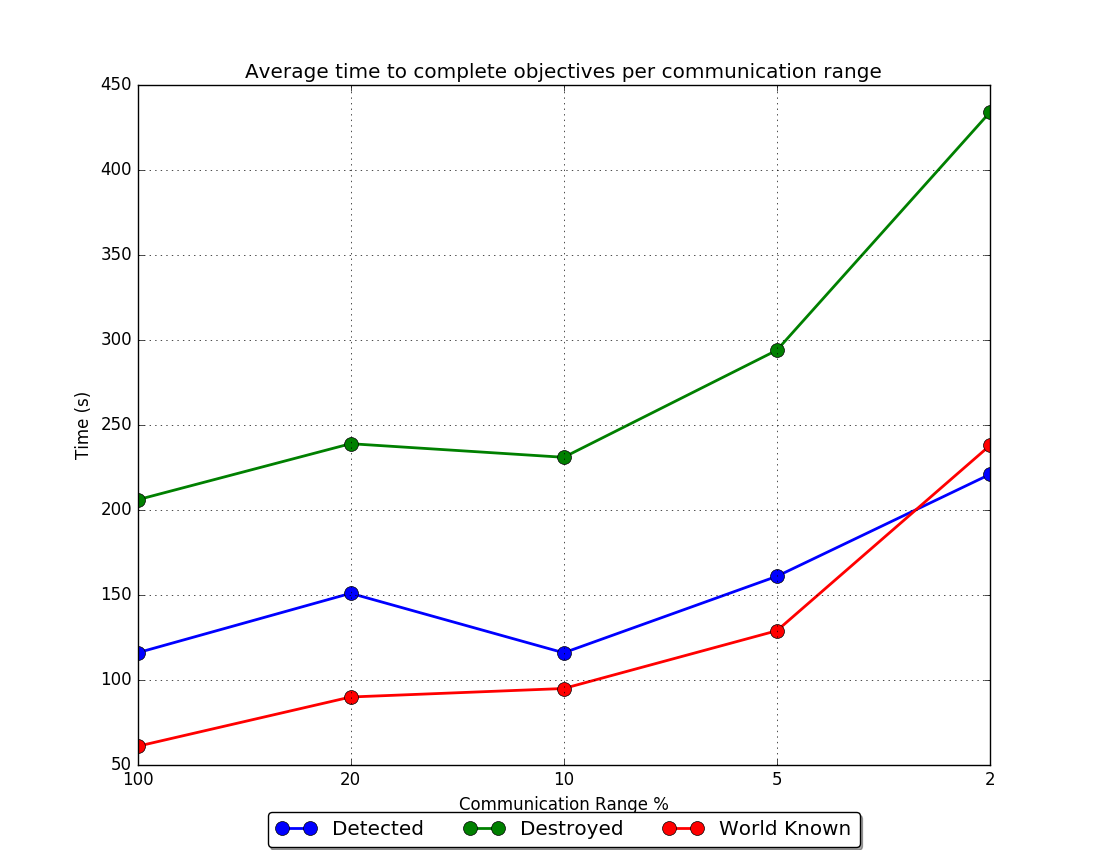
\includegraphics[width=\linewidth,height=4in,keepaspectratio=false]{averages.png}
	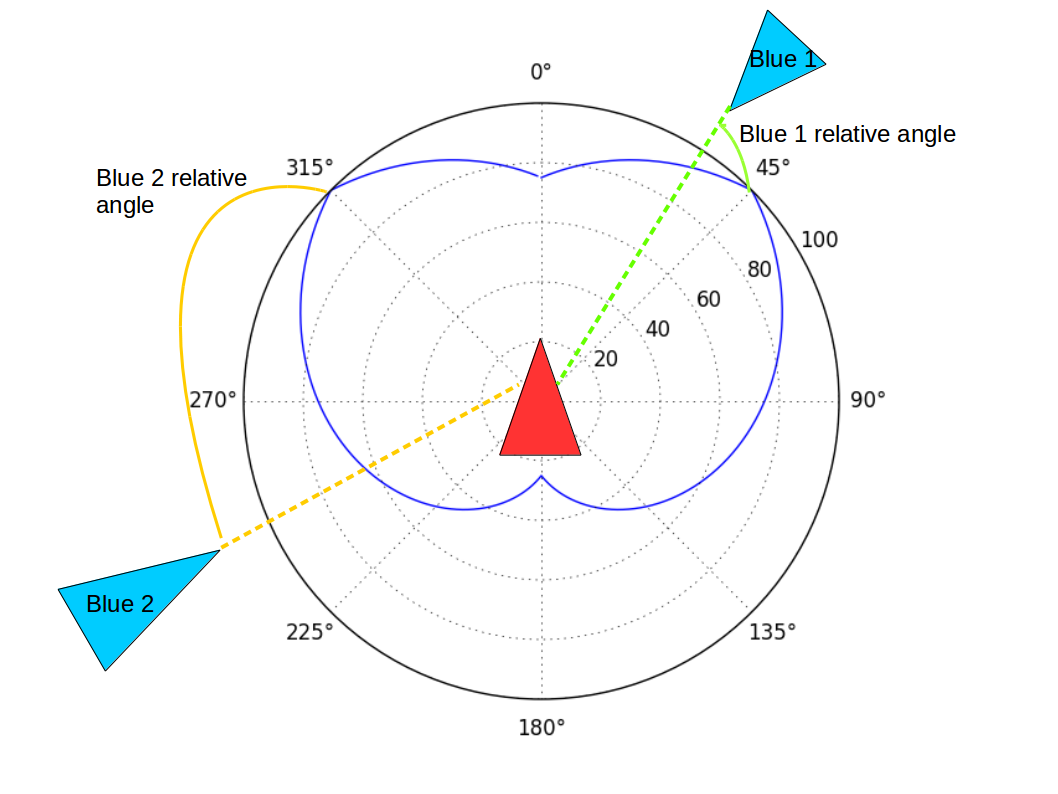
\includegraphics[scale=0.3]{blue_red_scale_angles.png}
	\caption{Success scaling per relative angles}
	\label{fig:blue_red_angles}
\end{figure}

%\begin{multicols*}{2}

\subsubsection{Detecting Empty Areas}
Not all areas in the world will contain a target.  Determining if an area is clear of targets has its own separate probability shown in Table~\ref{tab:snsrEmptyProb} where $P(S_{e}|T_{e})$ is the probability of detecting that an area is empty of targets given that the area really is empty of all targets.  Just because a sensor does not detect any targets at all does not mean the scanned area is clear of targets.  The sensor could have missed something or its line of sight may be occluded by an obstacle.

\begin{table}[H]
	\caption{Empty Cell Detection Probabilities}
	\centering
	\rowcolors{1}{lightgray}{white}
	\label{tab:snsrEmptyProb}
	%	\begin{tabular}{|p{1cm}|p{1cm}|}
	\begin{tabular}{|l|l|}
		\hline
		Sensor Type & $P(S_{e}|T_{e})$\\ \hline
		0 & 0.8\\ \hline
		1 & 0.6\\ \hline
	\end{tabular}
\end{table}

\subsubsection{Weapons}

Just like sensors, weapons have a lookup table containing the probability of successfully destroying a target assuming it is struck from its \textit{Best Angle}.  Any deviation from the \textit{Best Angle} causes a drop in the probability of destruction.  For example, let's imagine a car.  They have crumple zones to absorb impact energy to protect the occupants.  In a head-on collision the occupants are likely to survive because the front of the car will crumple and absorb a significant amount of energy.  If a car is struck along its sides in the door panels there is less protection for the occupants.  In this case the \textit{Best Angle} for a car is along the sides in the door panels. A sample set of data showing the probability of destruction mapping for each weapon and target combination in this experiment is shown in Table~\ref{tab:wpnTgtProb}.  $P(D_{x})$ is the probability of successfully destroying a target of type $x$.

\begin{table}[H]
	\caption{Weapon to Target Probabilities}
	\centering
	\rowcolors{1}{lightgray}{white}
	\label{tab:wpnTgtProb}
	\begin{tabular}{|p{1.5cm}|p{1.5cm}|p{3cm}|}
		\hline
%		 & Target Type & Prob(Destruction)\\ \hline
		Weapon Type & Target Type & $P(D_{x})$\\ \hline
		0 & 0 & 0.75 \\ \hline
		0 & 1 & 0.75 \\ \hline
		1 & 0 & 0.75 \\ \hline
		1 & 1 & 0.75 \\ \hline
	\end{tabular}
\end{table}

%\textbf{TODO: chance of misclassification. Chance of empty cell detection}


